
%	PACKAGES AND OTHER DOCUMENT CONFIGURATIONS
%----------------------------------------------------------------------------------------

\documentclass[
11pt, % The default document font size, options: 10pt, 11pt, 12pt
oneside, % Two side (alternating margins) for binding by default, uncomment to switch to one side
english, % ngerman for German
singlespacing, % Single line spacing, alternatives: onehalfspacing or doublespacing
%draft, % Uncomment to enable draft mode (no pictures, no links, overfull hboxes indicated)
%nolistspacing, % If the document is onehalfspacing or doublespacing, uncomment this to set spacing in lists to single
%liststotoc, % Uncomment to add the list of figures/tables/etc to the table of contents
%toctotoc, % Uncomment to add the main table of contents to the table of contents
%parskip, % Uncomment to add space between paragraphs
%nohyperref, % Uncomment to not load the hyperref package
headsepline, % Uncomment to get a line under the header
%chapterinoneline, % Uncomment to place the chapter title next to the number on one line
%consistentlayout, % Uncomment to change the layout of the declaration, abstract and acknowledgements pages to match the default layout
]{MastersThesis} % The class file specifying the document structure

\usepackage[utf8]{inputenc} % Required for inputting international characters
\usepackage[T1]{fontenc} % Output font encoding for international characters

\usepackage{palatino} % Use the Palatino font by default

\usepackage[autostyle=true]{csquotes} % Required to generate language-dependent quotes in the bibliography


\usepackage{url}
\usepackage{natbib} 
\usepackage{chapterbib}

%\addbibresource{SelectedReferences/BibReferences/MScThesisChapterI.bib} % The filename of the bibliography


%\usepackage[Sonny]{fncychap} % Options: Sonny, Lenny, Conny, Glenn, Rejne, Bjarne, Bjornstrup

\usepackage[]{quotchap}
%----------------------------------------------------------------------------------------
%	MARGIN SETTINGS
%----------------------------------------------------------------------------------------

\geometry{
	paper=a4paper, % Change to letterpaper for US letter
	inner=2.5cm, % Inner margin
	outer=2.5cm, % Outer margin
	bindingoffset=.5cm, % Binding offset
	top=1.5cm, % Top margin
	bottom=1.5cm, % Bottom margin
	%showframe, % Uncomment to show how the type block is set on the page
}

%----------------------------------------------------------------------------------------
%	THESIS INFORMATION
%----------------------------------------------------------------------------------------

\thesistitle{Detecting Blood Cells, Ultrasound Contrast Agent Micro-bubbles and Clusters Disturbed By Ultrasonic Filed from High Speed Photographs} % Your thesis title, this is used in the title and abstract, print it elsewhere with \ttitle
\supervisor{Dawit Assefa (PhD) \textsc{}} % Your supervisor's name, this is used in the title page, print it elsewhere with \supname
\examiner{} % Your examiner's name, this is not currently used anywhere in the template, print it elsewhere with \examname
\degree{Master of Science} % Your degree name, this is used in the title page and abstract, print it elsewhere with \degreename
\author{Mohammed Aliy\textsc{}} % Your name, this is used in the title page and abstract, print it elsewhere with \authorname
\addresses{} % Your address, this is not currently used anywhere in the template, print it elsewhere with \addressname

\subject{Biomedical Engineering} % Your subject area, this is not currently used anywhere in the template, print it elsewhere with \subjectname
\keywords{Segmentation, Red Blood Cell, Ultrasound, Microbubbles, Image Processing, Contrast Agent} % Keywords for your thesis, this is not currently used anywhere in the template, print it elsewhere with \keywordnames
\university{\href{http://www.aait.edu.et}{
		Addis Ababa University\\
		Addis Ababa Institute of Technology
		}} % Your university's name and URL, this is used in the title page and abstract, print it elsewhere with \univname
\department{\href{http://www.aait.edu.et}{
		Center of Biomedical Engineering\\
		Medical Imaging and Instrumentation Stream }} % Your department's name and URL, this is used in the title page and abstract, print it elsewhere with \deptname
\group{\href{http://researchgroup.university.com}{---}} % Your research group's name and URL, this is used in the title page, print it elsewhere with \groupname
\faculty{\href{http://faculty.university.com}{Faculty Name}} % Your faculty's name and URL, this is used in the title page and abstract, print it elsewhere with \facname

\AtBeginDocument{
\hypersetup{pdftitle=\ttitle} % Set the PDF's title to your title
\hypersetup{pdfauthor=\authorname} % Set the PDF's author to your name
\hypersetup{pdfkeywords=\keywordnames} % Set the PDF's keywords to your keywords
}

\begin{document}

\frontmatter % Use roman page numbering style (i, ii, iii, iv...) for the pre-content pages

\pagestyle{plain} % Default to the plain heading style until the thesis style is called for the body content

%----------------------------------------------------------------------------------------
%	TITLE PAGE
%----------------------------------------------------------------------------------------

\begin{titlepage}
\begin{center}


\includegraphics[scale=2]{AAU.png}\\
\vspace*{.01\textheight}
{\scshape\LARGE \univname\par}\vspace{1.5cm} % University name
\textsc{\Large Master Thesis}\\[0.5cm] % Thesis type

\HRule \\[0.4cm] % Horizontal line
{\huge \bfseries \ttitle\par}\vspace{0.4cm} % Thesis title
\HRule \\[1.5cm] % Horizontal line
 
\begin{minipage}[t]{0.4\textwidth}
\begin{flushleft} \large
\emph{Author:}\\
\href{}{\authorname} % Author name - remove the \href bracket to remove the link
\end{flushleft}
\end{minipage}
\begin{minipage}[t]{0.4\textwidth}
\begin{flushright} \large
\emph{Advisor:} \\
\href{}{\supname} % Supervisor name - remove the \href bracket to remove the link  
\end{flushright}
\end{minipage}\\[2cm]
 
\vfill

\large \textit{A thesis submitted in fulfillment of the requirements\\ for the degree of \degreename}\\[0.3cm] % University requirement text
\textit{in the}\\[0.4cm]
\groupname\\\deptname\\[2cm] % Research group name and department name
 
\vfill

{\large \today}\\[3cm] % Date
 % University/department logo - uncomment to place it
 
\vfill
\end{center}
\end{titlepage}

%----------------------------------------------------------------------------------------
%	DECLARATION PAGE
%----------------------------------------------------------------------------------------

\begin{declaration}
\addchaptertocentry{\authorshipname} % Add the declaration to the table of contents
\noindent I, \authorname, declare that this thesis titled, \enquote{\ttitle} and the work presented in it are my own. I confirm that:

\begin{itemize} 
\item This work was done wholly or mainly while in candidature for a research degree at this University.
\item Where any part of this thesis has previously been submitted for a degree or any other qualification at this University or any other institution, this has been clearly stated.
\item Where I have consulted the published work of others, this is always clearly attributed.
\item Where I have quoted from the work of others, the source is always given. With the exception of such quotations, this thesis is entirely my own work.
\item I have acknowledged all main sources of help.
\item Where the thesis is based on work done by myself jointly with others, I have made clear exactly what was done by others and what I have contributed myself.\\
\end{itemize}
 
\noindent Signed:\\
\rule[0.5em]{25em}{0.5pt} % This prints a line for the signature
 
\noindent Date:\\
\rule[0.5em]{25em}{0.5pt} % This prints a line to write the date
\end{declaration}

\cleardoublepage

%----------------------------------------------------------------------------------------
%	QUOTATION PAGE
%----------------------------------------------------------------------------------------

\vspace*{0.2\textheight}

\noindent\enquote{\itshape Thanks to my solid academic training, today I can write hundreds of words on virtually any topic without possessing a shred of information, which is how I got a good job in journalism.}\bigbreak

\hfill Dave Barry

%----------------------------------------------------------------------------------------
%	ABSTRACT PAGE
%----------------------------------------------------------------------------------------

\begin{abstract}
\addchaptertocentry{\abstractname} % Add the abstract to the table of contents
Blood cells and ultrasound contrast agent microbubbles show strange behaviors when they are subjected to ultrasound field. They migrate towards the nodes of the ultrasound wave and form a circular pattern. Time lapse of pattern formation is quite different between blood cells and ultrasound contrast agent microbubbles though. Ultrasound contrast agent microbubbles migrate towards the wave nodes very quickly and form a tightly packed clusters. In contrast, formation of tightly packed clusters in the case of blood cells is unlikely due to weak Bjerknes force and sonophore model of cells. To study such micron scale events (motility and shape sizing) of cells, especially red blood cells of near endothelial lining, there is a need to define a contour around the cells and determine their shape. To do so, first, cells (red blood cells) should be segmented from the rest of image content. In this regard, the main purpose of this thesis work is to devise a best cell segmentation technique that will perform well on the high speed photographs of such micron scale events. The thesis work will follow three procedures to narrow down the available cell segmentation techniques and come up with the best one; refining the available cell segmentation algorithms, testing the refined algorithms on the dataset and ranking the algorithms based on their subjective quality and lastly performing objective quality assessment of the images that performs good during visual image quality inspection and rank the best one or hybridize more than one algorithms.  The finding (ranked cell segmentation algorithm) will help to draw a contour line around red blood cells and study their mobility, interaction with each other and other particles and shape sizing when they are under ultrasound field.
\begin{center}
\line(1,0){250}
\end{center}

\textbf{Keywords: }\keywordnames
\end{abstract}

%----------------------------------------------------------------------------------------
%	ACKNOWLEDGEMENTS
%----------------------------------------------------------------------------------------

\begin{acknowledgements}
\addchaptertocentry{\acknowledgementname} % Add the acknowledgements to the table of contents
The acknowledgments and the people to thank go here, don't forget to include your project advisor\ldots
\end{acknowledgements}

%----------------------------------------------------------------------------------------
%	LIST OF CONTENTS/FIGURES/TABLES PAGES
%----------------------------------------------------------------------------------------

\tableofcontents % Prints the main table of contents

\listoffigures % Prints the list of figures

\listoftables % Prints the list of tables

%----------------------------------------------------------------------------------------
%	ABBREVIATIONS
%----------------------------------------------------------------------------------------

\begin{abbreviations}{ll} % Include a list of abbreviations (a table of two columns)

\textbf{LAH} & \textbf{L}ist \textbf{A}bbreviations \textbf{H}ere\\
\textbf{WSF} & \textbf{W}hat (it) \textbf{S}tands \textbf{F}or\\

\end{abbreviations}

%----------------------------------------------------------------------------------------
%	PHYSICAL CONSTANTS/OTHER DEFINITIONS
%----------------------------------------------------------------------------------------

\begin{constants}{lr@{${}={}$}l} % The list of physical constants is a three column table

% The \SI{}{} command is provided by the siunitx package, see its documentation for instructions on how to use it

Speed of Light & $c_{0}$ & \SI{2.99792458e8}{\meter\per\second} (exact)\\
%Constant Name & $Symbol$ & $Constant Value$ with units\\

\end{constants}

%----------------------------------------------------------------------------------------
%	SYMBOLS
%----------------------------------------------------------------------------------------

\begin{symbols}{lll} % Include a list of Symbols (a three column table)

$a$ & distance & \si{\meter} \\
$P$ & power & \si{\watt} (\si{\joule\per\second}) \\
%Symbol & Name & Unit \\

\addlinespace % Gap to separate the Roman symbols from the Greek

$\omega$ & angular frequency & \si{\radian} \\

\end{symbols}

%----------------------------------------------------------------------------------------
%	DEDICATION
%----------------------------------------------------------------------------------------

\dedicatory{For/Dedicated to/To my\ldots} 

%----------------------------------------------------------------------------------------
%	THESIS CONTENT - CHAPTERS
%----------------------------------------------------------------------------------------

\mainmatter % Begin numeric (1,2,3...) page numbering

\pagestyle{thesis} % Return the page headers back to the "thesis" style

% Include the chapters of the thesis as separate files from the Chapters folder
% Uncomment the lines as you write the chapters


% Chapter 1

\chapter{Introduction} % Main chapter title

\label{Chapter1} % For referencing the chapter elsewhere, use \ref{Chapter1} 

%----------------------------------------------------------------------------------------

% Define some commands to keep the formatting separated from the content 
\newcommand{\keyword}[1]{\textbf{#1}}
\newcommand{\tabhead}[1]{\textbf{#1}}
\newcommand{\code}[1]{\texttt{#1}}
\newcommand{\file}[1]{\texttt{\bfseries#1}}
\newcommand{\option}[1]{\texttt{\itshape#1}}

%----------------------------------------------------------------------------------------

\section{Background}

\setlength{\parindent}{10ex} Nearly three and half centuries passed since Antony Van Leeuwenhoek had drawn a benchmark for biological imaging by discovering “little animals ”, present day microbes, using his microscopes. His breakthrough paved a road to scientists and biologists to study tinny structures of living things. At that time, Leeuwenhoek’s main curiously was to magnify his “little animals”, protozoa and bacteria, and then study their structure though he was the first one to see and describe sperm and blood cells \cite{Croft2006,Dobell1960}. Since then, scientists and technologists have devoted and carried out remarkable works to magnify and study micro (small) level events and macro (large) level hidden or distant objects or structures. Micro level imaging technologies such as Scanning Probe Microscope (SPM), Transmission Electron Microscope (TEM) and Scanning Electron Microscope (SEM) help scientists and researchers to study immensely smaller resolution structures or objects \cite{Croft2006}.On the other hand, macro level imaging technologies such as X-ray, CT, MRI, PET, Ultrasound and SPECT help the physicians and researchers to understand anatomy and physiology of normal and abnormal internal hidden organs/tissues of human being \cite {Dhawan2011}. As well, macro level imaging technologies such as astrological telescopes help cosmologists to see distant cosmic objects \cite{Russ2016}.

The revolution of digital and information technology after the second half of the 20th century dominates the traditional analog way of imaging and simplify the method how images are acquired (both in time and process), processed, stored, displayed and transmitted from one place to the other. For example, these days, most molecular and cellular study laboratory microscopes have been integrated with high frame rate cameras. These high speed cameras will help the researcher to capture the photographs of cellular or molecular micron activities that are happened with in a fraction of second and store them for off-line studies.

The main purpose of this thesis work is to segment red blood cells of near to endothelial lining that are disturbed by ultrasonic energy and make them suitable for studying their micro activities.  The next subsection mainly focuses on image segmentation concepts such as types, commonly known techniques and challenges. Subsequently, discussions on preliminary concepts related to red blood cells, ultrasonic energy and microscale events of red blood cells near to endothelial lining will be presented. 

\begin{figure}[th]
	\centering
	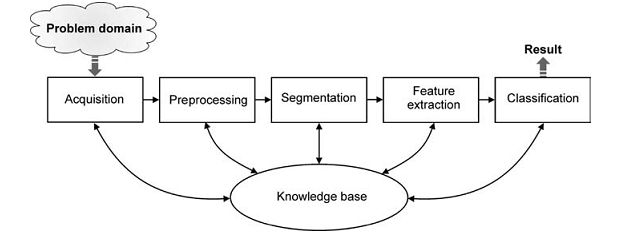
\includegraphics{Figures/computervisionsystem.png}
	%\decoRule
	\caption[Computer Vision System]{Computer vision system.}
	\label{fig:Computer Vision System}
\end{figure}


%----------------------------------------------------------------------------------------

\section{Statement of Problem}

Experimental results from previous work (Mazzawi et al., 2015) showed that sonication of mixture of blood, polystyrene microspheres and ultrasound contrast agent forces particles and cells  to migrate towards the nodes of the sound field. Particles and cells create a circular pattern as shown on Figure 5. When the sonication filed is halted the particles/cells trapped at the nodes remain there and the rest wobble inside the ring. All blood cells, ultrasound contrast agent and polystyrene microspheres are responsible for the circular pattern formation. However, ultrasound contrast agent microbubbles behave differently. They accumulate in circles at the nodes faster than blood cells and polystyrene microspheres and create a strong clusters as illustrated on Figure 6 which is not possible in blood cells and polystyrene particles due to weak Bjerknes forces. Besides, sonophore model of cells doesn’t allow strong cluster formation.
\begin{figure}[th]
	\centering
	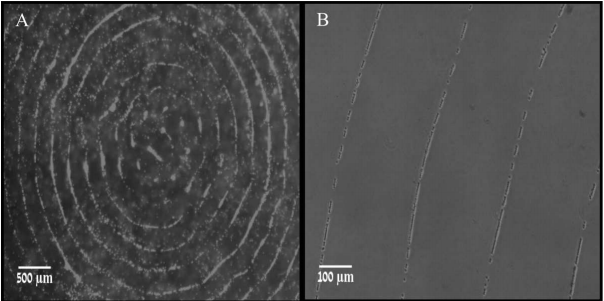
\includegraphics{Figures/CircularPattern.png}
	%\decoRule
	\caption[Circular Pattern Formation of Cells]{Ultrasound contrast agent (Quantison microbubbles) accumulated in circles(left) and form tightly packed cluster(right)}
	\label{fig:Circular Pattern Formation of Particles}
\end{figure}


\bibliographystyle{plain}
\bibliography{SelectedReferences/MScThesisChapterI}
% Chapter Template

\chapter{Ultrasound} % Main chapter title

\label{Chapter2} 

%----------------------------------------------------------------------------------------
%	SECTION 1
%----------------------------------------------------------------------------------------

\section{Overview}

This chapter gives a comprehensive summary of basics of Ultrasound field. Sections will discuss historical background of ultrasound, wave physics, generation of ultrasound wave artificially and application of ultrasound in medicine. 

\section{History}

Nunc posuere quam at lectus tristique eu ultrices augue venenatis. Vestibulum ante ipsum primis in faucibus orci luctus et ultrices posuere cubilia Curae; Aliquam erat volutpat. Vivamus sodales tortor eget quam adipiscing in vulputate ante ullamcorper. Sed eros ante, lacinia et sollicitudin et, aliquam sit amet augue. In hac habitasse platea dictumst.

\section{Wave Physics}
Morbi rutrum odio eget arcu adipiscing sodales. Aenean et purus a est pulvinar pellentesque. Cras in elit neque, quis varius elit. Phasellus fringilla, nibh eu tempus venenatis, dolor elit posuere quam, quis adipiscing urna leo nec orci. Sed nec nulla auctor odio aliquet consequat. Ut nec nulla in ante ullamcorper aliquam at sed dolor. Phasellus fermentum magna in augue gravida cursus. Cras sed pretium lorem. Pellentesque eget ornare odio. Proin accumsan, massa viverra cursus pharetra, ipsum nisi lobortis velit, a malesuada dolor lorem eu neque.


\section{Generation of Ultrasound}

Sed ullamcorper quam eu nisl interdum at interdum enim egestas. Aliquam placerat justo sed lectus lobortis ut porta nisl porttitor. Vestibulum mi dolor, lacinia molestie gravida at, tempus vitae ligula. Donec eget quam sapien, in viverra eros. Donec pellentesque justo a massa fringilla non vestibulum metus vestibulum. Vestibulum in orci quis felis tempor lacinia. Vivamus ornare ultrices facilisis. Ut hendrerit volutpat vulputate. Morbi condimentum venenatis augue, id porta ipsum vulputate in. Curabitur luctus tempus justo. Vestibulum risus lectus, adipiscing nec condimentum quis, condimentum nec nisl. Aliquam dictum sagittis velit sed iaculis. Morbi tristique augue sit amet nulla pulvinar id facilisis ligula mollis. Nam elit libero, tincidunt ut aliquam at, molestie in quam. Aenean rhoncus vehicula hendrerit.


\section{Medical Application of Ultrasound}

Sed ullamcorper quam eu nisl interdum at interdum enim egestas. Aliquam placerat justo sed lectus lobortis ut porta nisl porttitor. Vestibulum mi dolor, lacinia molestie gravida at, tempus vitae ligula. Donec eget quam sapien, in viverra eros. Donec pellentesque justo a massa fringilla non vestibulum metus vestibulum. Vestibulum in orci quis felis tempor lacinia. Vivamus ornare ultrices facilisis. Ut hendrerit volutpat vulputate. Morbi condimentum venenatis augue, id porta ipsum vulputate in. Curabitur luctus tempus justo. Vestibulum risus lectus, adipiscing nec condimentum quis, condimentum nec nisl. Aliquam dictum sagittis velit sed iaculis. Morbi tristique augue sit amet nulla pulvinar id facilisis ligula mollis. Nam elit libero, tincidunt ut aliquam at, molestie in quam. Aenean rhoncus vehicula hendrerit \cite{Dhawan2011}.

\bibliographystyle{plainnat}
\bibliography{SelectedReferences/MScThesisChapterI}





%---------------------------------------------------------------------------
%	THESIS CONTENT - APPENDICES
%---------------------------------------------------------------------------

\appendix % Cue to tell LaTeX that the following "chapters" are Appendices


% Appendix A

\chapter{Frequently Asked Questions} % Main appendix title

\label{AppendixA} % For referencing this appendix elsewhere, use \ref{AppendixA}

\section{How do I change the colors of links?}

The color of links can be changed to your liking using:

{\small\verb!\hypersetup{urlcolor=red}!}, or

{\small\verb!\hypersetup{citecolor=green}!}, or

{\small\verb!\hypersetup{allcolor=blue}!}.

\noindent If you want to completely hide the links, you can use:

{\small\verb!\hypersetup{allcolors=.}!}, or even better: 

{\small\verb!\hypersetup{hidelinks}!}.

\noindent If you want to have obvious links in the PDF but not the printed text, use:

{\small\verb!\hypersetup{colorlinks=false}!}.

%\include{Appendices/AppendixB}
%\include{Appendices/AppendixC}

\end{document}  

